\documentclass[12pt]{jarticle}
\usepackage{TUSIReport}
\usepackage{otf}
\usepackage{ascmac}
\usepackage{listings,jlisting}
\usepackage{url}
\usepackage[dvipdfmx]{graphicx}
\usepackage{here}
\usepackage{subfigure}
\usepackage{amssymb}
\usepackage{multirow}
\usepackage{longtable}
\setlength{\textwidth}{170mm}       % テキストの幅
\setlength{\textheight}{260mm}      % テキストの高さ
\setlength{\oddsidemargin}{-5mm}    % 偶数ページの左マージン
\setlength{\evensidemargin}{0mm}    % 奇数ページの左マージン
\setlength{\topmargin}{-25mm}       % 上のマージン  % 奇数ページの左マージン
\lstset{
  basicstyle={\ttfamily},
  identifierstyle={\small},
  commentstyle={\smallitshape},
  keywordstyle={\small\bfseries},
  ndkeywordstyle={\small},
  stringstyle={\small\ttfamily},
  frame={tb},
  breaklines=true,
  columns=[l]{fullflexible},
  numbers=left,
  xrightmargin=0zw,
  xleftmargin=3zw,
  numberstyle={\scriptsize},
  stepnumber=1,
  numbersep=1zw,
  lineskip=-0.5ex
}
\begin{document}
%%%%%%%%%%%%%%%%%%%%%%%%%%%%%%%%%%%%%%%%%%%%%%%%%%%%%%%%%%%%%%
% 表紙を出力する場合は,\提出者と\共同実験者をいれる
% \提出者{科目名}{課題名}{提出年}{提出月}{提出日}{学籍番号}{氏名}
% \共同実験者{一人目}{二人目}{..}{..}{..}{..}{..}{八人目}
%%%%%%%%%%%%%%%%%%%%%%%%%%%%%%%%%%%%%%%%%%%%%%%%%%%%%%%%%%%%%%
\提出者{情報工学実験2}{実験テーマ5 教育システム設計}{2020}{10}{5}{4619023}{加藤零}
\共同実験者{}{}{}{}{}{}{}{}

%%%%%%%%%%%%%%%%%%%%%%%%%%%%%%%%%%%%%%%%%%%%%%%%%%%%%%%%%%%%%%
% 表紙を出力しない場合は,以下の「\表紙出力」をコメントアウトする
%%%%%%%%%%%%%%%%%%%%%%%%%%%%%%%%%%%%%%%%%%%%%%%%%%%%%%%%%%%%%%
\表紙出力

%%%%%%%%%%%%%%%%%%%%%%%%%%%%%%%%%%%%%%%%%%%%%%%%%%%%%%%%%%%%%%
% 以下はレポート本体である.別途 TeXファイルを作成し \input 使っても良い
%%%%%%%%%%%%%%%%%%%%%%%%%%%%%%%%%%%%%%%%%%%%%%%%%%%%%%%%%%%%%%

\section{要旨}
高校で学習したベイズの定理が最尤推定を行う際にどのように応用されるかを学習・検討する.今回は,第一回及び第二回で利用した問いを複数個扱い対数関数を利用することで能力値を推定する.

\section{目的}
統計モデルを用いた分析は,商品の推薦や迷惑メールの削除機能など,身近な機能を支える基本的な技術となっている.本実験では,このような統計モデルを用いた分析に欠かせない,パラメタの推定の方法について基本的な技術を習得することを目的とする.

\section{理論}
\subsection{項目反応理論:複数問の反応からの能力値推定}
複数の問題に対する正誤反応を得た場合の能力値の推定について考える.今,ある問題系列について正誤反応${\bf X}_j=(x_{1,j},x_{2,j},...,x_{n,j})$が与えられたとする.この時の能力値$\theta$の推定値を考える際には以下のような数式を考えれば良い.
\begin{eqnarray}
    \hat{\theta}&=& \mathop{\rm arg~max}\limits_{\theta} P(\theta \mid {\bf X}_j)\\
    &=& \mathop{\rm arg~max}\limits_{\theta} P(\theta)P({\bf X}_j \mid \theta)
\end{eqnarray}
ここで$P({\bf X}_j \mid \theta)$はある能力値$\theta$の受験者が,それぞれの項目に${\bf X}_j)$のように反応する確率である.そのため,それぞれの項目への正誤が$\theta$のみに影響され定まるとすれば,$P({\bf X}_j \mid \theta)$は以下のようにかける.
\begin{eqnarray}
    P({\bf X}_j \mid \theta)&=&P(x_{1,j} \mid \theta)\times P(x_{2,j} \mid \theta) \times \cdots \times P(x_{n,j} \mid \theta)\\
    &=& \prod_{i=1}^n P(x_{i.j}\mid \theta)
\end{eqnarray}
つまり,複数のサイコロを同時に投げたときと同様に同時確率と見なすことができる.それぞれの項目への能力値$\theta$だけを媒介に独立に正誤反応していると考える.これを局所独立過程という.すなわち,それぞれの項目が他の項目の小rたえやヒントになっていない状況である.\\

また,$P(x_{i,j}\mid \theta)$は正答の場合と誤答の場合両方を以下のように表すことができる.
\begin{eqnarray}
    P(x_{i,j}\mid \theta)=P_i(\theta)^{x_{i,j}}\times (1-P_i(\theta))^{1-x_{i,j}}
\end{eqnarray}
従って考えるべき式は以下のようになる.
\begin{eqnarray}
    \hat{\theta}&=& \mathop{\rm arg~max}\limits_{\theta} P(\theta \mid {\bf X}_j)\\
    &=& \mathop{\rm arg~max}\limits_{\theta} P(\theta)\prod_{i=1}^n P(x_{i,j} \mid \theta)\\
    &=& \mathop{\rm arg~max}\limits_{\theta} P(\theta)\prod_{i=1}^n (P_i(\theta)^{x_{i,j}}(1-P_i(\theta))^{1-x_{i,j}})
\end{eqnarray}
ただし,これを計算機により計算機により計算することは,値域がをとる関数を複数回かけることになり,計算誤差が生じやすい.そのため,実装上は,このような関数の対数関数を考える.${\rm log}$は単調増加関数であり,ある関数$f(x)=x$が$x=x_{\rm max}$で最大を取るとき, ${\rm log}(f(x))$も$x=x_{\rm max}$で最大を取る.そのため,以下が成り立つ.
\begin{eqnarray}
    \hat{\theta}&=& \mathop{\rm arg~max}\limits_{\theta} P(\theta \mid {\bf X}_j)\\
    &=& \mathop{\rm arg~max}\limits_{\theta} \ln{(P(\theta \mid {\bf X}_j))}
\end{eqnarray}
そのため,実装上は以下を計算すれば良い.
\begin{eqnarray}
    \hat{\theta}=\mathop{\rm arg~max}\limits_{\theta} \Bigl\{\ln{(P(\theta))+\sum_{i=1}^n \Bigl(x_{i,j}\ln(P_i(\theta))+(1-x_{i,j})\ln(1-P_i(\theta))\Bigr)}\Bigr\}
\end{eqnarray}
これを対数尤度関数と呼ぶ.
\section{課題}
\subsection{課題3-1}
\begin{shadebox}
\end{shadebox}
\vspace{\baselineskip}

\subsection{課題3-2}
\begin{shadebox}
    \quad 課題1-3で解いた全ての項目の反応から自分の能力値$\theta$の対数尤度関数の概形を示せ.
\end{shadebox}
\vspace{\baselineskip}
私はitem1,4,7,10,13,16,19,22,25,28の10問について正答しており,結果は図3のようになった.先ほどの図2に着目してみると,正答した場合の対数尤度関数は誤答した場合の対数尤度関数に比べて右にずれていることがわかる.図3のグラフは式11の中括弧内の式を用いて描いたものであり,それぞれのitemに関して対数を取ったものの和を用いて表現している.今回問いに全問正解したことにより,各itemの対数尤度関数の山が右にずれ,その和で表される全体の対数尤度関数の山も右にずれたと推測できる.
\begin{figure}[H]
    \begin{center}
        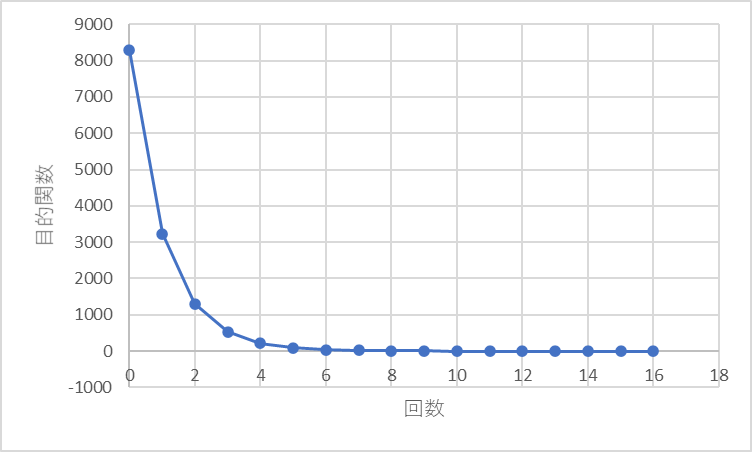
\includegraphics[bb=0 0 355 216,height=8cm]{3.png}
    \end{center}
    \caption{全ての項目による対数尤度}
    \label{fig1}
\end{figure}
\subsection{課題3-3}
\begin{shadebox}
    \quad 課題3-2で描いた対数尤度関数から能力値を推定せよ.またその時の情報量$I(\hat{\theta})$と標準誤差$se(\hat{\theta})$を求めよ.
\end{shadebox}
\vspace{\baselineskip}
図3において$\theta=1.3$の時に関数は最大値をとることから自分の能力値は1.3であると推定できる.今回の情報量は各itemに関する情報量の総和であるため以下の式を用いれば良い.
\begin{eqnarray*}
    I(\hat{\theta})&=&\sum_{i=1}^{10}{I_i({\theta})}\\
    &=&\sum_{i=1}^{10}{D^2a_i^2P_i(\theta)(1-P_i(\theta))}\\
    &=&\sum_{i=1}^{10}{1.7^2a_i^2P_i(1.3)(1-P_i(1.3))}\\
    &=&0.933706345\cdots\simeq 0.93371
\end{eqnarray*}
また,標準誤差は
\begin{eqnarray*}
    se(\hat{\theta})&=&I(\hat{\theta})^{-\frac{1}{2}}\\
    &=&\frac{1}{\sqrt{0.93371}}\\
    &=&1.03489156\cdots\simeq 1.03489
\end{eqnarray*}
となる.

\subsection{課題3–4}
\begin{shadebox}
    \quad 課題1-3で解いた項目の$a_i$が全て「1」だった場合の能力値,情報量,
    標準誤差を求め,結果について考察せよ.
\end{shadebox}
\vspace{\baselineskip}
グラフの概形は図4のようになった.また,図4より$\theta=1.1$のときに関数は最大値をとるため,能力値は1.1となり課題3-3と同様の計算を行うと情報量は約1.79014,標準誤差は約0.74741となった.グラフの概形は$a_i=1$でない時とほとんど変化がなく.これは困難度パラメタが変化していないためだといえる.情報量は課題3-3で$\sum_{i=1}^{10}{D^2a_i^2P_i(\theta)(1-P_i(\theta))}$によって与えられることが示されているが,今回はこの式の$a_i=1$となったことで情報量の総和が向上している.同様の理由で標準誤差は減少している.この結果は$a_i$が識別力パラメタを表しており,識別力パラメタが高いほど正答率が能力値に依存するという事実に沿っている.
\begin{figure}[H]
    \begin{center}
        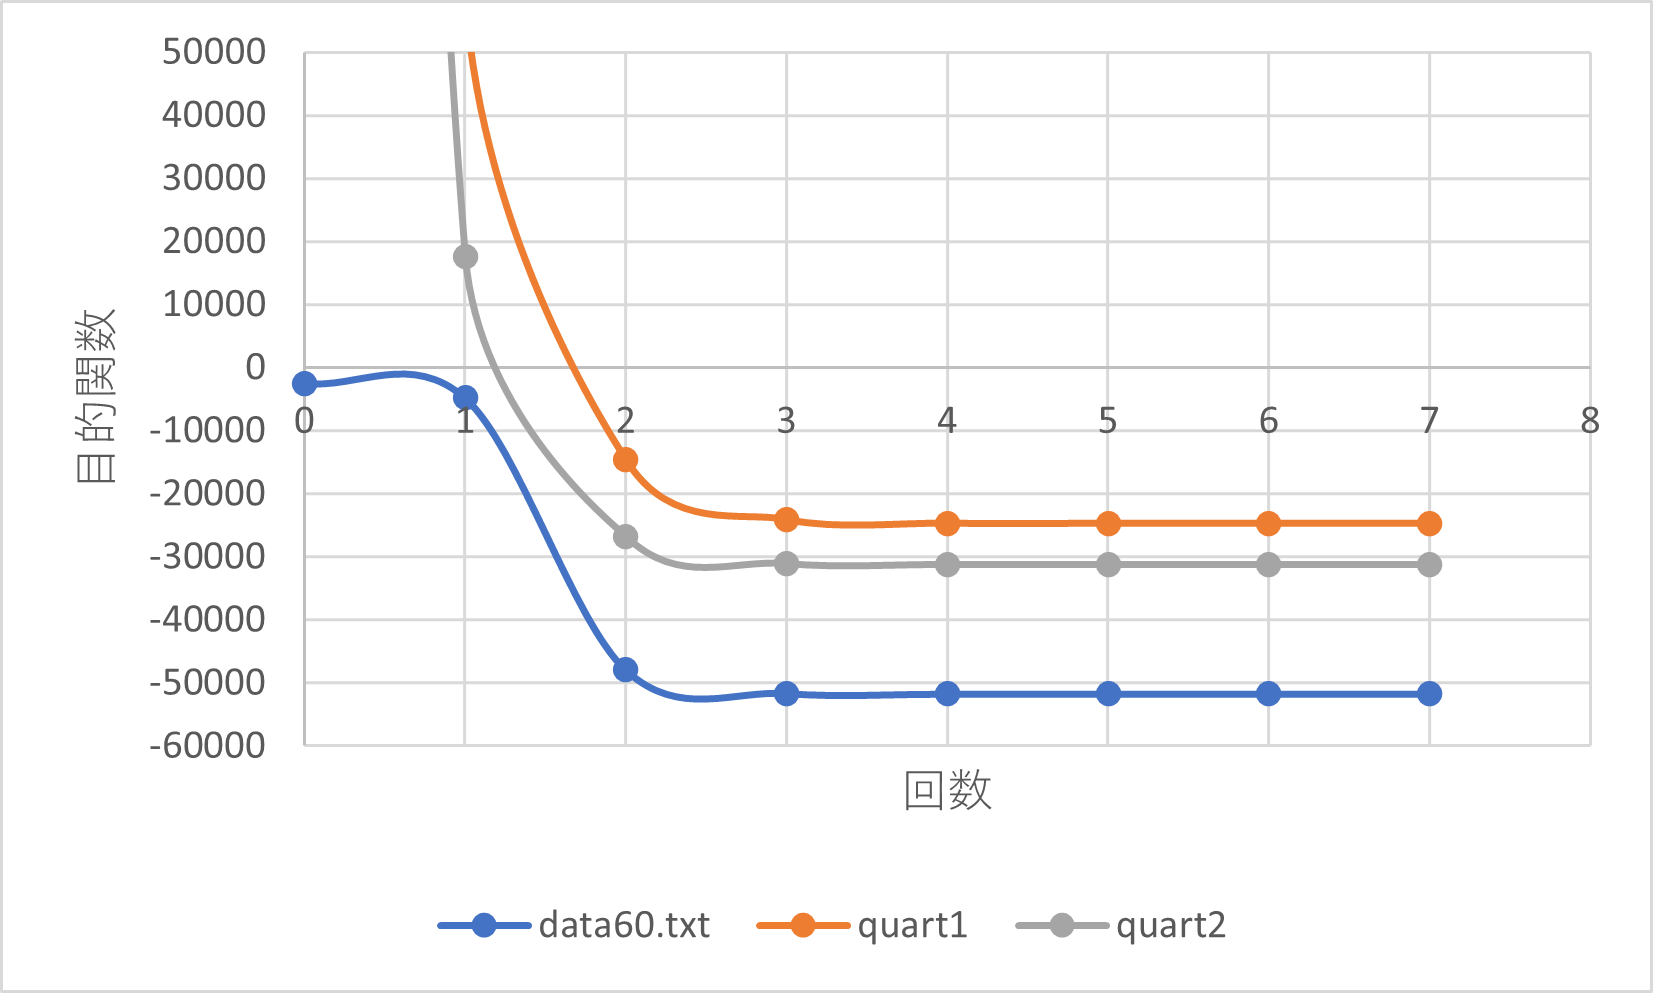
\includegraphics[bb=0 0 354 227,height=8cm]{4.png}
    \end{center}
    \caption{$a_i=1$のときの全ての項目による対数尤度}
    \label{fig1}
\end{figure}
\subsection{課題3–5}
\begin{shadebox}
    \quad 解いた項目と,能力値$\theta$の推定結果と,課題1-4で行なった偏差値$S$
    の結果を同じグループ内で共有し,比べた結果を考察せよ.
\end{shadebox}
\vspace{\baselineskip}
私のグループの結果をまとめると表1のようになった.尚,4618005はデータの提出がなかったため$?$として表記してある.今回はそれぞれの生徒が何点かという情報が与えられていなかったが,偏差値Sは以下の式12で与えられているため変形して式14を用いることで何点かを特定することができる.尚,平均点$u_x=60$で標準偏差$\sigma_x=15$である.
\begin{eqnarray}
    S&=&\frac{10(x-u_x)}{\sigma_x}+50\\
    x&=&\frac{\sigma_x(S-50)}{10}+u_x\\
    &=&\frac{3}{2}S-15
\end{eqnarray}
実際,表1の値はこれを利用して導出した.また,今回は解いた問題の合計を100点とし,一問あたりの点数は同じものとして扱うため,正答数も導出できる.4619023と4619050は得点は同じだが能力値が違うという事実から,同じ得点でも解いた問題数が多ければ能力値は向上すると言える.また,4619039の能力値が0.9となっているが,4619008や4619042,4619076と比較すると得点が低く解いている問題が少ないにもかかわらず,能力値が高くなっておりこの能力値が誤っているように感じる.実際,この条件で能力値が0.9になるためには全問正解している必要があったので4619039の能力値に誤りがあることが判明した.このように能力値や偏差値,得点,正答数などを並べた上でデータを眺めることで誤りに気づくことができる.
\begin{table}[h]
    \begin{center}
        \centering
        \caption{班員の解答結果}
        \begin{tabular}{|c|r|r|r|r|r|r|r|r|} \hline
            学籍番号                     & \multicolumn{1}{|c|}{4619008} & \multicolumn{1}{|c|}{4619023} & \multicolumn{1}{|c|}{4619039} & \multicolumn{1}{|c|}{4619042} & \multicolumn{1}{|c|}{4619050} & \multicolumn{1}{|c|}{4619076} & \multicolumn{1}{|c|}{4619086} & \multicolumn{1}{|c|}{4618005} \\
            \hline
            能力値                       & 0.6                           & 1.3                           & 0.9                           & 0.7                           & 1.0                           & 0.6                           & 0.0                           & ?                             \\ \hline
            偏差値                       & 63.3                          & 76.7                          & 60.0                          & 63.3                          & 76.6                          & 63.3                          & 56.7                          & ?                             \\ \hline
            \multirow{20}{*}{解いた問題} & 4                             & 1                             & 7                             & 1                             & 7                             & 1                             & 2                             & ?                             \\
                                         & 12                            & 4                             & 10                            & 5                             & 10                            & 4                             & 3                             & ?                             \\
                                         & 20                            & 7                             & 23                            & 7                             & 13                            & 7                             & 5                             & ?                             \\
                                         & 36                            & 10                            & 47                            & 11                            & 38                            & 10                            & 7                             & ?                             \\
                                         & 44                            & 13                            &                               & 12                            & 46                            & 13                            & 11                            & ?                             \\
                                         &                               & 16                            &                               & 16                            &                               &                               & 13                            & ?                             \\
                                         &                               & 19                            &                               & 19                            &                               &                               & 17                            & ?                             \\
                                         &                               & 22                            &                               & 23                            &                               &                               & 19                            & ?                             \\
                                         &                               & 25                            &                               & 25                            &                               &                               & 23                            & ?                             \\
                                         &                               & 28                            &                               & 28                            &                               &                               & 29                            & ?                             \\
                                         &                               &                               &                               & 31                            &                               &                               & 31                            & ?                             \\
                                         &                               &                               &                               & 34                            &                               &                               & 37                            & ?                             \\
                                         &                               &                               &                               & 35                            &                               &                               & 41                            & ?                             \\
                                         &                               &                               &                               & 40                            &                               &                               & 43                            & ?                             \\
                                         &                               &                               &                               & 44                            &                               &                               & 47                            & ?                             \\
                                         &                               &                               &                               &                               &                               &                               & 48                            & ?                             \\
                                         &                               &                               &                               &                               &                               &                               & 40                            & ?                             \\
                                         &                               &                               &                               &                               &                               &                               & 50                            & ?                             \\
                                         &                               &                               &                               &                               &                               &                               & 51                            & ?                             \\
                                         &                               &                               &                               &                               &                               &                               & 52                            & ?                             \\ \hline
            得点                         & 80                            & 100                           & 75                            & 80                            & 100                           & 80                            & 70                            & ?                             \\ \hline
            正答数                       & 4                             & 10                            & 3                             & 12                            & 5                             & 4                             & 14                            & ?                             \\ \hline
        \end{tabular}
    \end{center}
\end{table}
\clearpage
\subsection{課題3c–1}
\begin{shadebox}
    \quad 課題1-3で解いた全ての項目での対数尤度関数に対
    して,ニュートン法を用いて能力値を推定せよ.
\end{shadebox}
\vspace{\baselineskip}
今回は以下に示すnewton.pyを利用して推定した.利用したプログラミング言語はPythonである.ニュートン法は$\theta_{k+1}=\theta_k-\frac{f'(\theta)}{f(\theta)}$によって$k+1$の点を導出できる.これは,以下の式によって示されている.
\begin{eqnarray*}
    f'(\theta)&=&\frac{dy}{d\theta}\\
    &=&\frac{f(\theta)}{\theta_k-\theta_{k+1}}\\
    \theta_k-\theta_{k+1}&=&\frac{f(\theta)}{f'(\theta)}\\
    \theta_{k+1}&=&\theta_k-\frac{f'(\theta)}{f(\theta)}
\end{eqnarray*}
式11を用いることで能力値を推定できることがわかるため,今回はニュートン法を用いるにあたって$f(\theta)$を式11の中かっこ内として利用すればよい.これはnewton.pyの29行目から36行目の関数で利用している.次に$f(\theta)$を$\theta$によって微分して導関数を求める.今回はわかりやすくするため,項ごとに微分する.すると以下のようになる.
\begin{eqnarray*}
    \frac{d}{d\theta}\ln(P(\theta))&=&\frac{d}{d\theta}\ln\left(\frac{1}{\sqrt{2\pi}}\exp\left(-\frac{\theta^2}{2}\right)\right)\\
    &=&-\theta\\
    \frac{d}{d\theta}x_{i,j}\ln(P_i(\theta))&=&\frac{d}{d\theta}x_{i,j}\ln\left(\frac{1}{1+\exp\{-Da_i(\theta_j -b_i)\}}\right)\\
    &=&x_{i,j}\frac{Da_i\exp\{-Da_i(\theta_j -b_i)\}}{1+\exp\{-Da_i(\theta_j -b_i)\}}\\
    \frac{d}{d\theta}(1-x_{i,j})\ln(1-P_i(\theta))&=&\frac{d}{d\theta}(1-x_{i,j})\ln\left(\frac{\exp\{-Da_i(\theta_j -b_i)\}}{1+\exp\{-Da_i(\theta_j -b_i)\}}\right)\\
    &=&(1-x_{i,j})\frac{-Da_i}{1+\exp\{-Da_i(\theta_j -b_i)\}}
\end{eqnarray*}
これらを組み合わせると式11の中括弧内の関数の導関数は
\begin{eqnarray*}
    -\theta+\sum_{i=1}^n\left({x_{i,j}\frac{Da_i\exp\{-Da_i(\theta_j -b_i)\}}{1+\exp\{-Da_i(\theta_j -b_i)\}}+(1-x_{i,j})\frac{-Da_i}{1+\exp\{-Da_i(\theta_j -b_i)\}}}\right)
\end{eqnarray*}
となる.これはnewton.pyの39行目から47行目の関数で利用している.尚,ニュートン法では$\theta=-4$からだけでなく$\theta=4$の方向からも推定した.実行結果は次のようになった.
\clearpage

\begin{lstlisting}[title=newton.pyの実行結果(左から)]
    θ = -4
    f(θ) = -39.821791010861304
    f'(θ) = 12.590610179993595
    
    θ = -0.8371833897186418
    f(θ) = -9.346867331156279
    f'(θ) = 5.610655901430599
    
    θ = 0.8287300962203239
    f(θ) = -4.016506024989266
    f'(θ) = 1.0437954052759046
  \end{lstlisting}
\begin{lstlisting}[title=newton.pyの実行結果(右から)]
    θ = 4
    f(θ) = -9.251500859407221
    f'(θ) = -3.7877094120056394
    
    θ = 1.557494555922537
    f(θ) = -3.8066551046799604
    f'(θ) = -0.41476248433076995
  \end{lstlisting}
以上の結果より,$\theta$が0.82873から1.55749の間にあると推定できる.実際,課題3-3で能力値が約1.3であると判明しているので推定は正当であるといえる.

\begin{lstlisting}[title=newton.py,label=kadai1]
    import math

    a = [0.39117,
        0.32597,
        0.6118,
        0.33723,
        0.67552,
        0.89931,
        0.64296,
        0.47439,
        0.34592,
        0.63141, ]
    b = [-0.74843,
        0.03162,
        -0.48178,
        -0.63348,
        -0.57458,
        -1.14805,
        0.20626,
        -0.11113,
        -1.07541,
        -1.70127]
    D = 1.7
    question = [1]*10  # 正答した問題は1,間違いは0
    theta = 4  # どこの点からニュートン法を利用するか
    limit = 0.0001
    
    
    def func(theta):  # 対数尤度
        res = math.log((1/math.sqrt(2*math.pi))*math.exp(-(theta**2)/2))  # 標準正規分
        for k in range(len(question)):
            if question[k]:  # 正答の場合
                res += math.log(1/(1+math.exp(-D*a[k]*(theta-b[k]))))
            else:  # 誤答の場合
                res += math.log(1-1/(1+math.exp(-D*a[k]*(res-b[k]))))
        return res
    
    
    def derivativeFunc(theta):  # 次の方向
        res = -theta  # 標準正規分布の導関数の初期値
        for k in range(len(question)):
            if question[k]:  # 正答の場合
                res += (D*a[k]*math.exp(-D*a[k]*(theta-b[k]))) / \
                    (1+math.exp(-D*a[k]*(theta-b[k])))
            else:  # 誤答の場合
                res += -D*a[k]/(1+math.exp(-D*a[k]*(theta-b[k])))
        return res
    
    
    result = []
    tmp = 0
    while(True):
        result.append({"θ": theta, "f(θ)": func(theta),
                      "f'(θ)": derivativeFunc(theta)})
        tmp = theta
        theta -= func(theta)/derivativeFunc(theta)
        if abs((theta-tmp)/tmp) < limit or theta > 4 or theta < -4:  # 終了条件
            break
    for el in result:
        for key in list(el.keys()):
            print(key+' = '+str(el[key]))
        print()
    
  \end{lstlisting}
\section{まとめ}
今回の演習・課題により項目反応理論を複数の項目について適用し能力値を推定することでより確からしい能力値が取得できるということがわかった.また,対数関数を利用することで通常積の形で表される関数を和で表すことができるようになり,関数の性質を保持したまま導関数を導出するのが容易になった.また,今回のニュートン法により能力値の推定は真値に近いが一致はしなかった.

% 参考文献
\begin{thebibliography}{99}
    \label{sannkoubunnkenn_chapter}
    \bibitem{} 数値解析入門: Newton法\\
    \url{http://pen.envr.tsukuba.ac.jp/~nishida/lecture/numerical/Newton.html}\\
    最終閲覧日; 2020/10/11
    \bibitem{} 項目反応理論(Item Response Theory:IRT)に関連する用語説明 Ver1.1\\
    \url{http://www.med.oita-u.ac.jp/mededuc/cbt/riron_yougo.pdf}\\
    最終閲覧日; 2020/10/11
\end{thebibliography}

%%%%%%%%%%%%%%%%%%%%%%%%%%%%%%%%%%%%%%%%%%%%%%%%%%%%%%%%%%%%%%
\end{document}
